% SPDX-License-Identifier: CC-BY-SA-4.0
% Author: Matthieu Perrin
% Part: 
% Section: 
% Sub-section: 
% Frame: 

\begingroup

\begin{frame}{Théorème d'équivalence entre AFN et AFD}
  \SetKwData{Input}{motif}

  \vspace{-1.5cm}
  \begin{minipage}{4.8cm}
    \begin{block}{Théorème}
      Tout langage reconnaissable par un automate fini  non-déterministe 
      est reconnaissable par un automate fini déterministe
    \end{block}
  \end{minipage}

  \vspace{1.3cm}
  \begin{block}{Démonstration}
    Méthode des sous-ensembles de Rabin et Scott
    \begin{description}
    \item [Entrée :] automate fini non-déterministe \structure{$A$}
    \item [Sortie :] automate fini déterministe \structure{$B$} tel que $\mathcal{L}(B) = \mathcal{L}(A)$ 
      \begin{itemize}
      \item les états de $B$ sont des ensembles d'états de $A$ 
      \item $B$ est également complet
      \end{itemize}
    \end{description}
  \end{block}

  \vspace{-7.4cm}\hspace\fill
  \begin{minipage}{2.7cm}
    \centering
    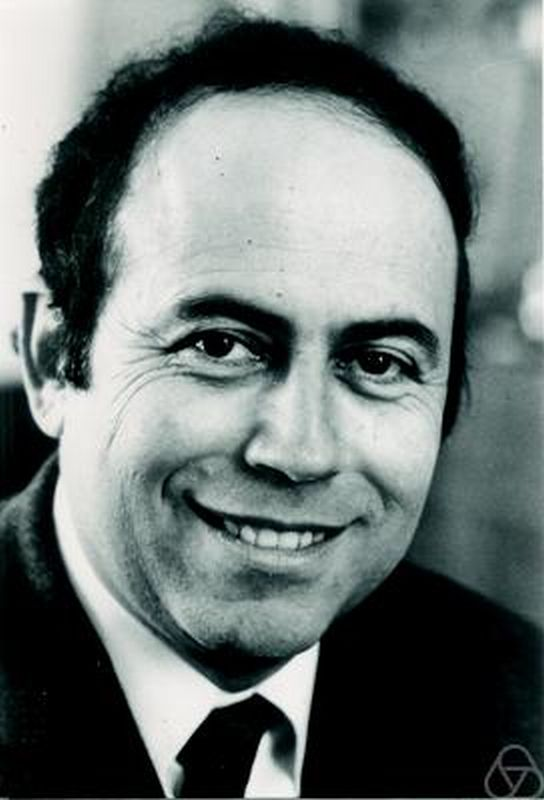
\includegraphics[height=4cm]{img/Rabin}
    
    Michael O. Rabin${}^1$
  \end{minipage}\hspace{2mm}
  \begin{minipage}{2.7cm}
    \centering
    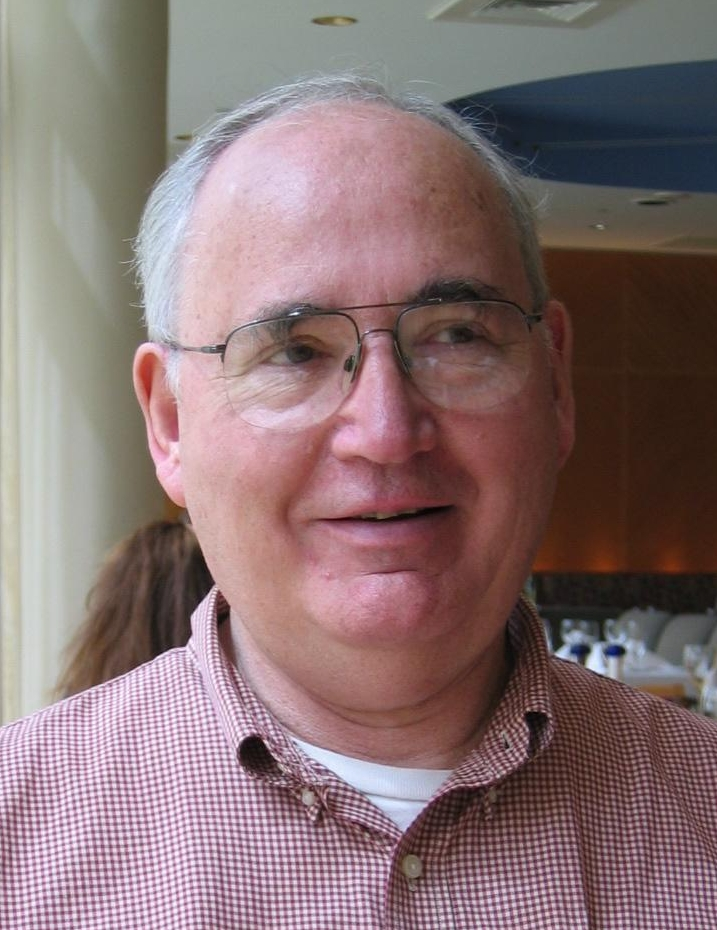
\includegraphics[height=4cm]{img/Scott}
    
    Dana S. Scott\footnote[frame,1]{Prix Turing 1976 pour leurs travaux sur le non-déterminisme}
  \end{minipage}
\end{frame}

\endgroup
